%zu "untersuchen". Mir geht es persönlich darum, wie dieses Produkt
%im realen Alltag einzusetzen ist und wie es technisch funktioniert
%(whitepaper lesen/überfliegen!).

%Dafür hätte ich gerne ein Tutorial, das genau diese Punkte als
%"Tutorial"
%behandelt, sodass ich dieses im Unterricht (unter Linux) einsetzen
%könnte.
%Speziell interessant ist der Einsatz in einem Container.
\chapter{WireGuard}
\begin{figure}[htbp]
  \centering
  \includesvg[scale=0.20]{images/wireguard.svg}
  \caption{WireGuard Logo}
\end{figure}

\section{Einführung} % Was kann ich damit machen?
\label{einfuehrung}
WireGuard ist ein extrem einfaches und dennoch schnelles und modernes VPN-Protkoll, welches eine sichere Lösung für das VPN-Tunneling bieten soll. Es ist darauf ausgelegt, leistungsfähiger, einfacher und nützlicher als die Konkurrenz z.B. IPsec, OpenVPN  zu sein. WireGuard ist als Allzweck-VPN konzipiert, das sowohl auf eingebetteten Schnittstellen als auch auf Supercomputern ausgeführt werden kann und für viele verschiedene Umstände geeignet ist.  \newline\newline
Ursprünglich wurde WireGuard für den Linux-Kernel veröffentlicht, ist jedoch nun plattformübergreifend (Windows, MacOS, BSD, iOS, Android) weitgehend einsetzbar. Derzeit wird WireGuard stark weiterentwickelt, aber kann jetzt schon als die sicherste, benutzerfreundlichste und einfachste VPN-Lösung in der Branche angesehen werden.

\section{Installation} 
\label{installation}
WireGuard kann wie in Abschnitt \ref{einfuehrung} beschrieben, auf vielen Betriebssystemen eingesetzt werden. Die Installation wird in weiterer Folge für das Betriebssystem Linux erklärt. \newline\newline
Unter Ubuntu $\geq$ 19.10 erfolgt die Installation durch:
\begin{lstlisting}
$ sudo apt install wireguard
\end{lstlisting}
Ubuntu $\leq$ 19.04:
\begin{lstlisting}
$ sudo add-apt-repository ppa:wireguard/wireguard
$ sudo apt-get update
$ sudo apt-get install wireguard
\end{lstlisting}

\newpage  \noindent
Debian:
\begin{lstlisting}
# apt install wireguard
\end{lstlisting}
Arch:
\begin{lstlisting}
$ sudo pacman -S wireguard-tools
\end{lstlisting}

\section{Verwendung} % Einsatz im Realen Alltag
Im folgenden Abschnitt werde ich auf alle Schritte eingehen, die zur Installation von WireGuard notwendig waren. Klar, es gibt immer mehrere Wege zu einem Ziel.
\subsection{Vorbereitung} 
\label{vorbereitung}
Um eine sinnvolle Funktionalität von WireGuard zu demonstrieren ist sowohl ein Server, als auch ein Client notwendig. Dazu habe ich in der Oracle Virtualbox zwei virtuelle Maschinen aufgesetzt. Auf einer VM lief ein \href{https://ubuntu.com/download/server}{Ubuntu Server} mit der Version 18.04.4, auf der anderen VM lief ein \href{https://ubuntu.com/download/desktop}{Ubuntu Desktop System} mit der Version 19.10. Der Vorgang zum Aufsetzen, erfolgt wie üblich. Ich empfehle lediglich dem Client mehr als 1GB RAM zuzuweisen, da er sonst während der Installation abstürzen kann. Zusätzlich sollte man die neueste Version von VirtualBox installieren, da in älteren Versionen offiziell Bugs bei der Kommunikation zwischen den VMs bestehen. Dies kann sonst einige Stunden Aufwand kosten :) .\newline
Da zur Verwendung von WireGuard eine Kommunikation zwischen Client und Server und zum Internet notwendig ist, müssen ein paar Konfigurationen in der VirtualBox vorgenommen werden. Dazu muss bei beiden VMs auf den Netzwerk Adaptern \textit{NAT} ausgewählt sein (default). Beim Ubuntu Server muss man einen zusätzlichen Netwerkadapter aktivieren und ihn als \textit{Host-only} Adapter einstellen. \newline
\begin{figure}[H]
  \centering
  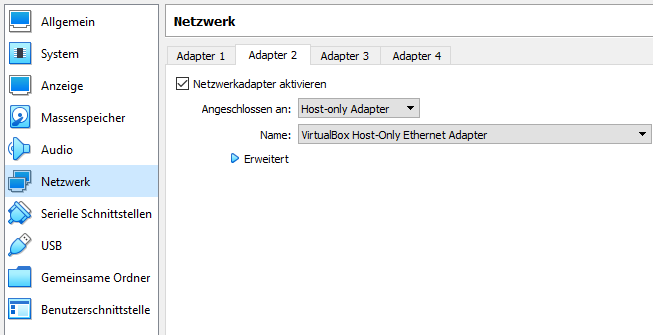
\includegraphics[scale=0.75]{images/vm-nw.png}
  \caption{Host-only Adapter}
\end{figure} \noindent
Es wird davon abgeraten ein eigenes NAT-Network zu konfigurieren, da in VirtualBox somit zwar eine Kommunikation zwischen den VMs funktioniert, jedoch keine Kommunikation zum Internet, wordurch keine Installation von WireGuard möglich ist. \newpage \noindent
Anschließend muss diesem neu angelegten Adapter eine IP-Adresse zugewiesen werden. Der Name des Adapters kann mit dem Befehl \textit{ifconfig -a} identifiziert werden. Unser gewünschter Adapter ist derjenige, der keine IP Adresse besitzt. In meinem Fall war das \textit{enp0s8}. Dazu kann mit dem Befehl 
\begin{lstlisting}
$ vi /etc/network/interfaces
\end{lstlisting}
dem Adapter folgenderweise eine IP-Adresse zugewiesen werden:
\begin{lstlisting}
auto enp0s8
iface enp0s8 inet static
address 192.168.56.10
netmask 255.255.255.0
\end{lstlisting}
Zuletzt kann wieder der Befehl \textit{ifconfig} ausgeführt werden, der Folgendes zurückliefert:
\begin{figure}[H]
  \centering
  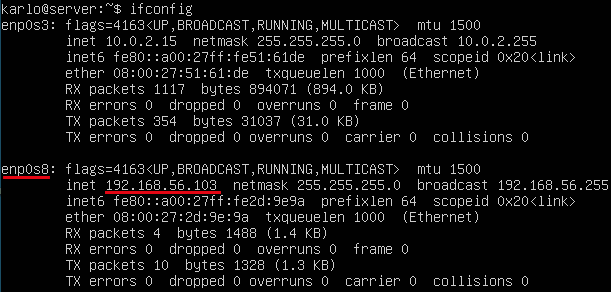
\includegraphics[scale=0.7]{images/ifconfig.PNG}
  \caption{IP Adressen der Netzwerkadapter}
\end{figure} \noindent
\subsection{Server}
Sind nun die Schritte aus Abschnitt \ref{vorbereitung} ausgeführt, kann die Installation von WireGuard beginnen. Dazu sind der Server und der Client zu starten. Um WireGuard am Server zu installieren ist am Client folgender Befehl auszuführen:
\begin{lstlisting}
$ ssh <username>@192.168.56.103
\end{lstlisting}
Anschließend wurde mit folgenden Befehlen WireGuard am Server installiert:
\begin{lstlisting}
add-apt-repository ppa:wireguard/wireguard
apt-get update
apt-get install wireguard-dkms wireguard-tools linux-headers-$(uname -r)
\end{lstlisting}
Danach wurde mit folgenden Befehlen ein private und public Key generiert:
\begin{lstlisting}
umask 077
wg genkey | tee server_private_key | wg pubkey > server_public_key
\end{lstlisting}
\newpage \noindent
Um die Konfigurationen langfristig zu speichern kann mit dem Befehl
\begin{lstlisting}
$ vi /etc/wireguard/wg0.conf
\end{lstlisting}
eine Konfigurationsdatei erstellt werden, die folgenden Inhalt enthält:
\begin{lstlisting}
[Interface]
Address = 10.100.100.1/24
SaveConfig = true
PrivateKey = 
ListenPort = 51820
PostUp = iptables -A FORWARDls -i %i -j ACCEPT; iptables -A FORWARD -o %i -j ACCEPT; iptables -t nat -A POSTROUTING -o eth0 -j MASQUERADE

PostDown = iptables -D FORWARD -i %i -j ACCEPT; iptables -D FORWARD -o %i -j ACCEPT; iptables -t nat -D POSTROUTING -o eth0 -j MASQUERADE

[Peer]
PublicKey = 
AllowedIPs = 10.100.100.2/32
\end{lstlisting}
In Zeile 4 tragen wir den generierten Private Key des Servers ein. Zeile 11 bleibt vorerst so wie sie ist. \newline\newline
Anschließend muss noch IPv4 forwarding erlaubt werden, um den Zugriff auf das gesamte LAN zu ermöglichen.
Dazu ist folgender Befehl auszuführen:
\begin{lstlisting}
$ vi /etc/sysctl.conf
\end{lstlisting}
und in folgender Zeile den Befehl:
\begin{lstlisting}
net.ipv4.ip_forward=1
\end{lstlisting}
auszukommenntieren. \newline\newline
Um diese Änderungen zu übernehmen kann entweder der Server mit dem Befehl \textit{reboot} neugestartet werden, oder mit folgenen Befehlen ohne eines Neustarts übernommen werden:
\begin{lstlisting}
sysctl -p
echo 1 > /proc/sys/net/ipv4/ip_forward
\end{lstlisting} \noindent
Soweit so gut. Der Server ist nun konfiguriert. \newline\newline
WireGuard kann nun mit folgenden Befehl gestartet werden:
\begin{lstlisting}
$ wg-quick up wg0
\end{lstlisting}
Möchte man, dass WireGuard automatisch gestartet wird, sobald der Server gestartet wird, kann man das mit folgenden Befehl erreichen:
\begin{lstlisting}
$ systemctl enable wg-quick@wg0.service 
\end{lstlisting}
\newpage
\subsection{Client}
Zuerst muss WireGuard installiert werden. Dieser Vorgang ist in Abschnitt \ref{installation} erklärt. Für Ubuntu 19.10 habe ich folgenden Befehl ausgeführt:
\begin{lstlisting}
$ sudo apt install wireguard
\end{lstlisting} 
 Anschließend wird für den Client ein private und public Key generiert.
\begin{lstlisting}
wg genkey | tee client_private_key | wg pubkey > client_public_key
\end{lstlisting}
Nun muss noch in der Server Konfigurationsdatei in Zeile 11 der Public Key des Clients eingetragen werden. \newline\newline
Zuletzt wird wieder eine Konfigurationsdatei angelegt.
\begin{lstlisting}
$ vi /etc/wireguard/wg0-client.conf
\end{lstlisting}
Diese hat folgenden Inhalt:
\begin{lstlisting}
[Interface]
Address = 10.100.100.2/32
PrivateKey =

[Peer]
PublicKey =
Endpoint = :51820
AllowedIPs = 0.0.0.0/0
PersistentKeepalive = 21
\end{lstlisting}
In Zeile 3 wird der Private Key des Clients eingetragen und in Zeile 6 der Public Key des Servers. Zeile 7 enthält zusätzlich noch die IP Adresse des Servers. \newline
Wireguard ist nun am Client konfiguriert und kann mit folgenden Befehl gestartet werden:
\begin{lstlisting}
$ sudo wg-quick up wg0-client
\end{lstlisting}
Überprüft man nun die IP Adresse des Clients, stellt man fest, dass die IP Adresse des WireGuard Servers zu sehen ist, anstelle der ursprünglichen IP Adresse des Clients. \newline
Führt man den Befehl
\begin{lstlisting}
$ sudo wg-quick down wg0-client
\end{lstlisting}
aus erhält man wieder die ursprüngliche IP Adresse des Clients.
\newpage
\section{Technische Funktionalität}